\documentclass[titlepage]{article}[11pt]

\usepackage{amsmath}
\usepackage{graphicx, float}
\usepackage[font=small,labelfont=bf]{caption}
\usepackage{subfig}
\usepackage{url}
\usepackage{hyperref}
\usepackage{natbib}
\usepackage{braket}
\usepackage{stix}
\usepackage{bm}
\usepackage[separate-uncertainty = true]{siunitx}
\usepackage[a4paper, top=1.5cm, bottom=2cm, left=1.5cm, right=1.5cm]{geometry}
\nocite{*}

\renewcommand{\abstractname}{\large Abstract} 

\begin{document}

\begin{titlepage}
	\centering
	
	\title{Simulation studies of different detector designs for the ePIC Silicon Vertex Tracker}

	\author{\parbox{\linewidth}{\centering%
		\textbf{Candidate Number:} 1616771 \endgraf
		\textbf{Project Number:} B8\_04 \endgraf
		\textbf{Supervisor:} Dr Samuel Henry \endgraf
		}}

	\maketitle

\end{titlepage}

\begin{center}
	{\Large \textbf{Abstract}}
\end{center}
\begin{list}{}{
	\leftmargin=1cm  
	\rightmargin=1cm  
}
\item 
Silicon tracking detectors are now a ubiquitous part of high energy particle physics experiments. The simulation of different detector designs is an important step to ensure the final design can achieve the required level of tracking precision. In this project, I developed a detector simulation and track reconstruction workflow to study how design choices affect the expected performance of the ePIC Silicon Vertex Tracker (SVT). I simulated the passage of single positive pions through a simplified SVT geometry in Geant4, and reconstructed tracks from detector hit positions using a helical fit. The fitted track parameters were compared with the true simulated values to extract momentum, position, and angular resolutions in order to investigate the impacts of detector design choices such as intrinsic hit resolution, detector material thickness and magnetic field strength. The results show that increasing the material budget worsens the resolution across all momenta, improving the hit resolution only benefits tracking resolution for high momentum, and increasing the magnetic field only improves momentum resolution.
\end{list}

\section{Introduction} \label{Introduction}
Tracking and vertex detectors allow for the reconstruction of trajectories for charged particles in a magnetic field. This allows scientists to determine the momenta, charge, and vertex positions of different particles produced in high energy collisions, making them an essential component for collider experiments. The most common type of detectors for this purpose are made from silicon diodes, which create electrical signals when ionising particles travel through the detector. Silicon vertex trackers can be made to have extremely high spatial resolution, as they can be segmented into strips or pixels on the order of micrometres. They also have fast response times, high efficiency, low levels of noise, and can be made to have a low material budget, reducing the impact of scattering, allowing for more accurate tracking. 

The focus of this report is the Silicon Vertex Tracker which is slated for construction as part of the future ePIC (Electron-Proton/Ion Collider) experiment at Brookhaven National Laboratory, which will take place in the 2030s. The experiment will collide polarised beams of electrons and ions/protons to study the properties of quarks and gluons inside visible matter, such as their 3D distribution in nuclei, and how they contribute to the proton spin. In order to achieve these goals, the ePIC experiment requires extremely precise measurements of charged particle momenta and vertex positions, with specific resolution requirements specified in the EIC Yellow Report \cite{ABDULKHALEK2022122447}. 

The accuracy of a tracking detector depends strongly on its geometry, and so it is important to simulate and evaluate different detector layouts in order to find the optimal design. The aim of this project is to construct a computational workflow for detector performance studies, and use it to demonstrate how different design choices affect tracking performance, using the SVT as a case study. I implemented a simplified model of the ePIC SVT in Geant4, generated positive pions travelling through the detector, and reconstructed particle trajectories to detector hit positions using a helical fit. I then compared the reconstructed track parameters with the known truth values from the simulation to measure tracking resolution. Using this framework, I investigated how the resolution changes when varying the intrinsic detector resolution, material thickness, and magnetic field strength.

\section{Geant4 detector simulation} \label{Method}

This section outlines the computational procedure for simulating particles in the SVT using Geant4, which is a C++ toolkit that is commonly used in many nuclear and particle physics applications \cite{Geant4}. Geant4 allows the user to specify the physical layout of an experiment, including the materials and geometry, and then simulates the passage of particles and radiation through the geometry. Geant4 tracks the movement of particles in discrete steps and uses Monte Carlo methods to solve the necessary particle transport equations, accounting for different physical effects that alter the trajectory of particles and result in the creation of secondary particles. These effects might include electromagnetic interactions, hadronic interactions, particle decay and interactions with electric and magnetic fields, depending on which physics has been specified in the simulation\footnote[1]{
	All simulations mentioned in this report use the standard \texttt{FTFP\_BERT} physics list.
}. Geant4 also handles the detector response, allowing for hit information to be exported, and also contains many other features useful for simulation, such as visualisation, run management, and interaction with the application via a user interface or macro commands. 

\subsection{SVT detector geometry}

\begin{figure}[H]
	\centering
	\includegraphics[width=1\linewidth]{ePIC_SVT_diagram}
	\caption{A diagram of the ePIC Central Detector with the tracking detector magnified and the SVT components labelled}
	\label{fig:epicsvtdiagram}
\end{figure}

As shown in Figure \ref{fig:epicsvtdiagram}, the SVT comprises the innermost detector layer in the ePIC experiment, being situated immediately outside of the beampipe to be as close as possible to the collision vertices. The SVT contains 5 cylindrical detector layers covering the central pseudorapidity\footnote[2]{
	The pseudorapidity $\eta$ of a particle is related to $\theta$, the angle of the particle's momentum relative to the positive $z$-axis and is defined as $\eta = -\ln \left[ \tan \left(\frac{\theta}{2}\right) \right]$. A pseudorapidity of 0 corresponds to a particle travelling perpendicular to the $z$-axis, a pseudorapidity approaching $\infty$ corresponds to a particle travelling in the positive $z$ direction, and a pseudorapidity approaching $-\infty$ corresponds to a particle travelling in the negative $z$ direction.
} range ($-1 \leq \eta \leq 1$), consisting of 3 inner barrel (IB) layers made from curved silicon sensors, and 2 outer barrel (OB) layers made from segmented staves. There are also an additional 10 disk shaped layers covering the high pseudorapidity regions ($1 \leq |\eta| \leq 3.5$), with 5 electron endcaps (EE) and 5 hadron endcaps (HE). The detector layers are constructed using Monolithic Active Pixel Sensor (MAPS) technology, which combines the sensor and readout electronics into the same silicon substrate. These allow for a low material budget and high spatial resolution, with the sensors having a thickness of \qty{50}{\micro \metre}, and a pixel size of $21 \times 23$ \unit{\micro \metre \squared}. The sensors also use minimal power, allowing for air cooling, minimising the amount of support structures required for electronics and cooling that would contribute to the total material budget. 

A simplified model of the ePIC SVT was constructed in Geant4 that approximates the main detector dimensions without incorporating finer details. The model includes the silicon detector layers as shown in Figure \ref{fig:detectorlayout}, approximated as basic cylindrical or disk-shaped volumes instead of detailed stave structures. The dimensions were chosen according to the most recent geometry description of the ePIC experiment on GitHub\footnote[3]{
	Geometry Description of the ePIC Experiment. Available at: \url{https://github.com/eic/epic} [Accessed \today]
}. It should be noted that the endcap discs are positioned slightly asymmetrically, which results in asymmetrical tracking performance in the forward and backward regions. This is intentional, to account for the asymmetrical distribution of pseudorapidities of secondary particles due to the vastly different energies of the electron and ion beams (\qty{18}{\giga \electronvolt} and \qty{275}{\giga \electronvolt} respectively). The model also includes a uniform magnetic field of \qty{1.7}{\tesla} along the positive $z$ direction, and a hollow beryllium beampipe with a radius of \qty{31}{\milli \metre} and a thickness of \qty{0.757}{\milli \metre} containing vacuum inside. 

\begin{figure}[H]
	\centering
	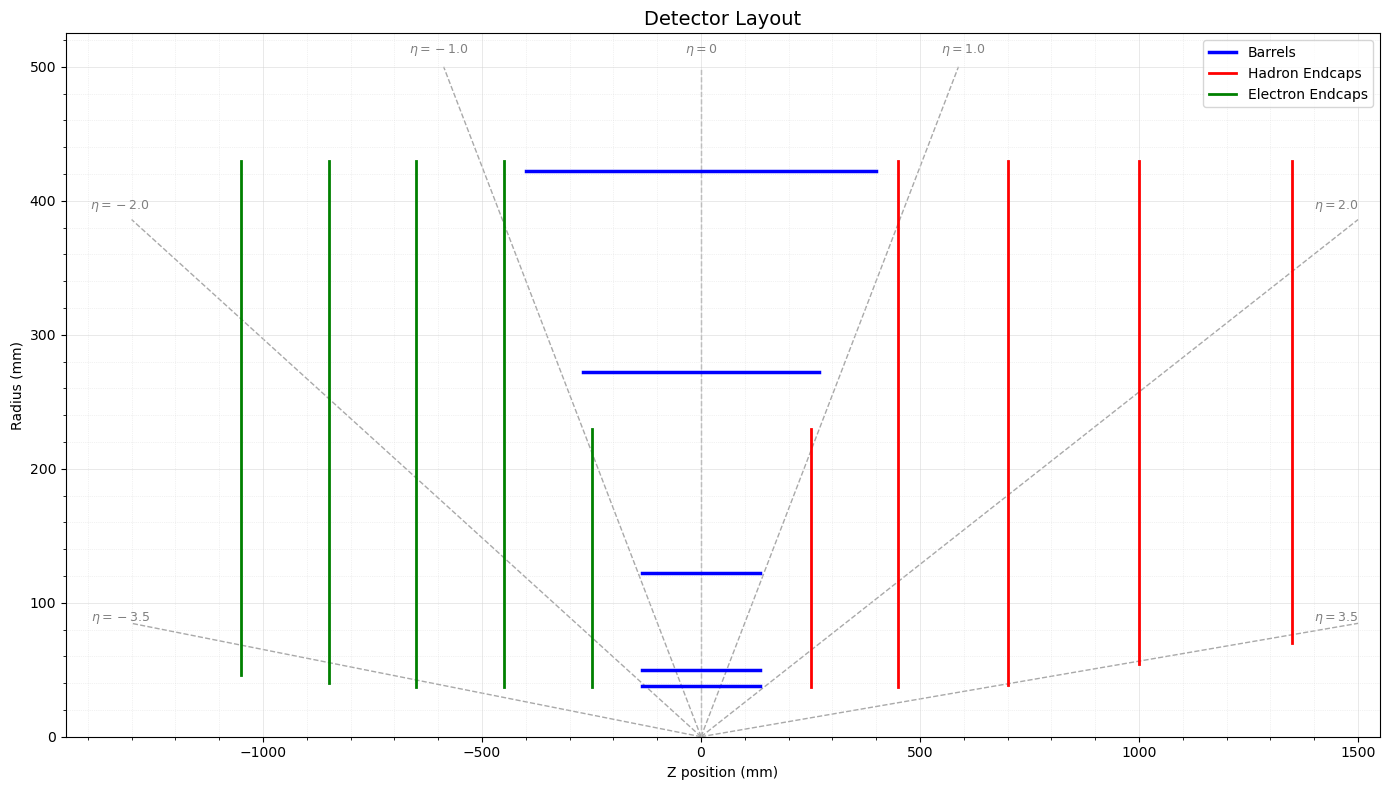
\includegraphics[width=0.8\linewidth]{detector_layout}
	\caption{$rz$-diagram of the simulated detector layout with lines of constant pseudorapidity indicated}
	\label{fig:detectorlayout}
\end{figure}

The silicon thickness was fixed at \qty{50}{\micro \metre}. Layers of copper material were placed sandwiching the silicon to approximate the impact of supporting material. The thickness of the copper was determined such that the combined radiation length \footnote[4]{
	The radiation length $X_0$ describes the typical thickness of material required to reduce the energy of a relativistic electron to $\frac{1}{e}$ of its original energy. 
} of the silicon and copper matched the total planned material budget of the specified layer. The goal was to replicate the impacts of multiple Coulomb scattering, which causes deviations to the trajectory of charged particles. Since this effect depends primarily on the radiation length, the shape and type of supporting material are less important than the overall material thickness per layer. Therefore, I chose to use simple layers of copper instead of precisely modelling the cooling, readout and mechanical support structures, which are made of many different materials such as carbon-fibre, nylon and aluminium. Copper was chosen as a representative support material, as it is a common material found in the electrical components of the SVT.

\subsection{Particle generation}
In order to gain some understanding of the types of particles that might be produced in a typical collision at the EIC, and therefore which particles would be useful to simulate, a Pythia8 simulation of a \qty{275}{\giga \electronvolt} proton and \qty{18}{\giga \electronvolt} electron collision was performed. Pythia8 is a C++ program to simulate the results of high energy particle collisions according to the current theoretical models and phenomenological descriptions of high-energy collisions \cite{Pythia8}.

 \begin{figure}[H]
 	\centering
 	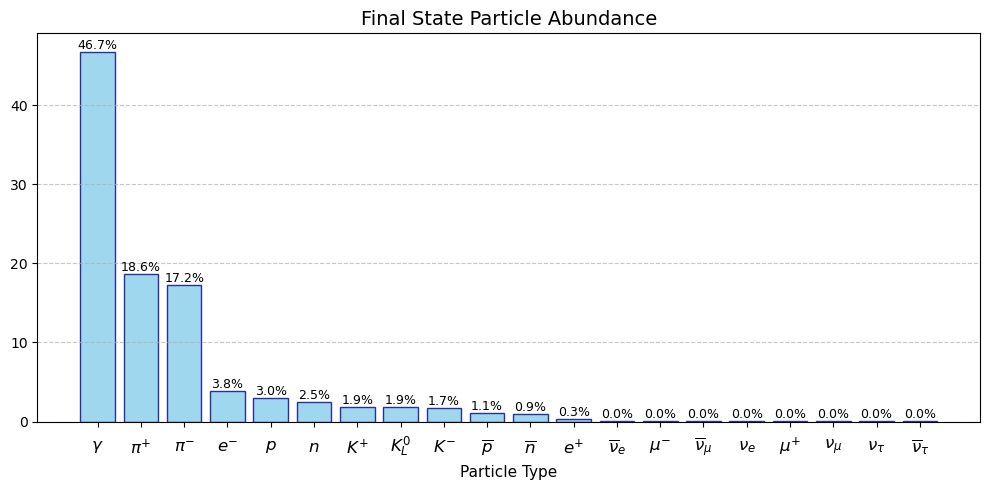
\includegraphics[width=0.7\linewidth]{particle_abundances}
 	\caption{Frequency of final state particles produced in the $p + e^-$ collision according to the Pythia8 simulation}
 	\label{fig:particleabundances}
 \end{figure}
 
 \noindent
 A histogram of the most common particles produced in a sample size of 1000 collisions is shown above in Figure \ref{fig:particleabundances}. Photons are the most commonly produced particles, however they will usually leave no trace in the silicon detectors as they are neutral. Therefore in my simulations, I chose to use positive pions, as pions are the most common type of charged particles. I used the \verb|G4ParticleGun| class, which allows for the creation of individual particles with an initial position and momentum. Pions were emitted from the origin, with a uniform distribution of pseudorapidities from $-3.5 \leq \eta \leq 3.5$, and with a wide range of magnitudes of momentum from \qty{150}{\mega \electronvolt} to \qty{20}{\giga \electronvolt}.  
 
\begin{figure}[H]
	\centering
	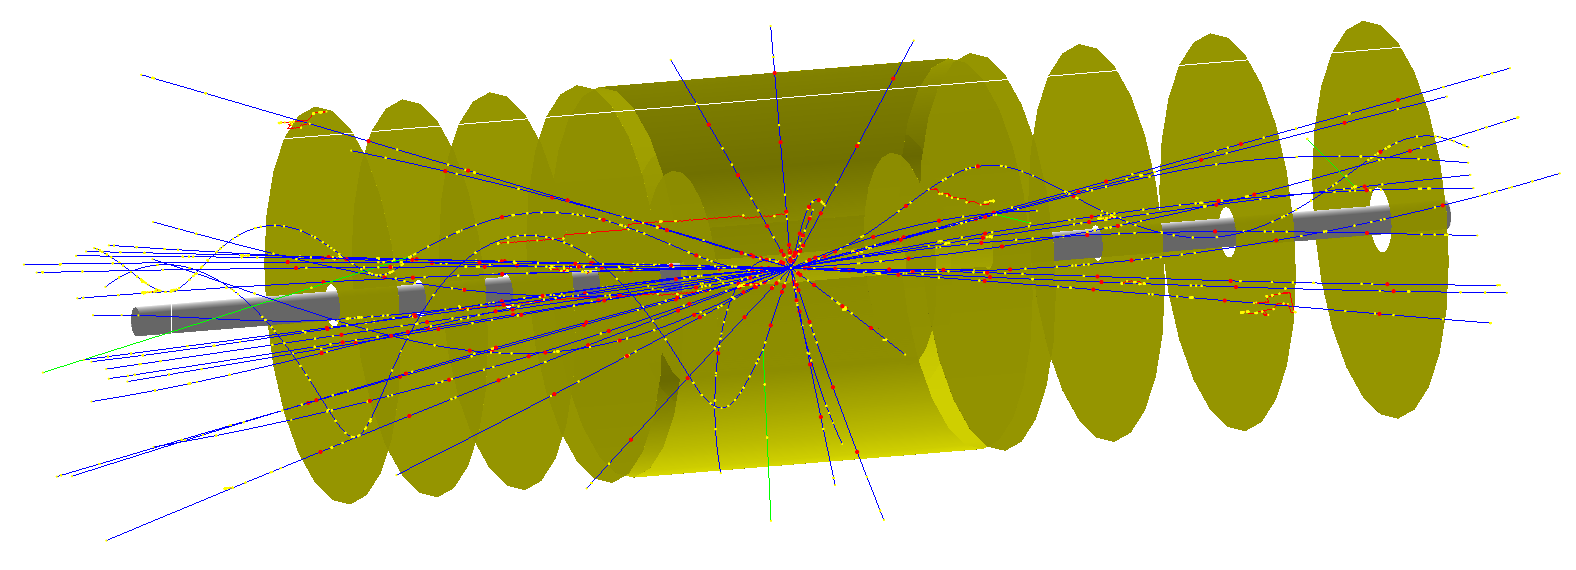
\includegraphics[width=1\linewidth]{geant4_screenshot}
	\caption{An example visualization showing the result of simulating 50 positive pions through the detector in Geant4. The yellow volumes correspond to the detector layers and the grey volume corresponds to the beampipe. The blue, green and red curves correspond to the tracks left by positive, neutral and negative particles respectively. Yellow dots indicate discrete simulation steps, while red dots represent detector hits.}
	\label{fig:geant4screenshot}
\end{figure}


\subsection{Detector Hits}
When constructing the silicon volumes in Geant4, I used the \verb|G4VSensitiveDetector| class, which triggers the \verb|ProcessHits| method whenever a particle steps through the volume. The \verb|ProcessHits| method checks if the energy deposited is above some threshold, which is supposed to match the physical operating principle of a real detector. In a silicon detector charged particles ionise the material, creating electron-hole pairs. These electrons drift toward collection diodes, and the stored charge is converted into a readout voltage. Typically there is a charge threshold of a couple hundred electrons, in order to avoid detecting fake hits from noise. In my simulation, I decided to set the threshold to \qty{1}{\kilo \electronvolt}, which is on the order of a few hundred electron-hole pairs. 

In a real detector, there will be uncertainty in the hit position due to charge diffusion and digitisation. After a hit produces hundreds of electron-hole pairs, the electrons will drift randomly, depositing different amounts of charge on multiple nearby pixels. The hit position is taken to be the centroid position of the activated pixels. There is also an uncertainty in position due to the finite size of each pixel. In this simulation, I make the simplifying assumption that the combined effects of charge diffusion, clustering and pixelation can be modelled by a single Gaussian measurement uncertainty, with a standard deviation of $\sigma=\qty{7}{\micro \metre}$, consistent with the estimated resolution of the SVT sensors \cite{turrisi2026epicsiliconvertextracker}. 

For the endcap discs, this is implemented by applying independent Gaussian smearing to the $x$ and $y$ coordinates of each hit. For the barrel layers, it is more natural to work in cylindrical coordinates: the radial coordinate is left unchanged, while Gaussian smearing is applied independently to the $z$-coordinate and the azimuthal coordinate $\phi$. The smearing in $\phi$ is chosen such that the corresponding uncertainty in the tangential direction $r \phi$ is equal to \qty{7}{\micro \metre}, i.e. $\sigma_\phi = \sigma / r$.

As shown in Figure \ref{fig:geant4screenshot}, the emitted pions produce many secondary particles such as photons and electrons after colliding with the beampipe, detector material, or air. In practice, these secondary particles could potentially result in other detector hits which don't follow the primary particle track, making the next task of track reconstruction much more difficult. For simplification, I only record hits which correspond to the primary pions emitted by the particle gun. The smeared detector hit positions are exported to a ROOT\footnote[5]{
	ROOT is a file format used by the ROOT data analysis framework (available at \url{https://root.cern/}), which was developed by CERN and is commonly used in particle physics for scientific data analysis of large quantities of data.
} file, along with an identifier indicating which pion produced the hit, and the generated initial momentum of this pion (which will be used later to compare the reconstructed momentum against). 

\section{Track reconstruction and resolution measurement}
Track reconstruction is the process of reconstructing particle trajectories or "tracks" from detector hits, which allows for the momentum and vertex position to be determined. In this section, I take the detector hits produced from each individual pion and fit a helical trajectory to the hit positions. I use these helices to estimate the initial momentum and position, and compare these to the truth values in order to evaluate the momentum and position uncertainty of the detector. In practice, the raw experimental data would include the hits from all particles produced after several collisions, and there would be an additional challenge of matching which hits correspond to which tracks, known as "track finding". For the purposes of this report, I am only interested in the intrinsic tracking resolution, and not how efficiently hits can be matched to tracks, since this typically depends less on the detector design and more on the type of algorithm used. Therefore, for simplification, I skip this track finding step, assuming that hits have already been labelled with the corresponding track.

\subsection{Motion of charged particles in a magnetic field}
A charged particle in a uniform magnetic field experiences a Lorentz force $F = q(\vec{v} \times \vec{B})$ that causes it to move in a helical trajectory. The coordinates are set so that the magnetic field and the beamline (the axis along which the electron and ion beams are oriented) are parallel to the $z$-axis with $\vec{B} = B \hat{z}$. After solving the equations of motion, we find that the particle moves in circular motion in the $xy$-plane, and moves along the $z$ direction at a constant rate. It is useful to parametrise the helical motion with 5 parameters $\left(d_0, \phi_0, z_0, p_T, \tan \lambda \right)$, corresponding to physically significant quantities. Defining the point of closest approach (POCA) as the point when the particle is closest to the $z$-axis, then the parameters correspond to the following:

\begin{itemize}
	\item $d_0$ is the transverse distance in the $xy$-plane from the particle to the z-axis at the POCA.
	\item $z_0$ is the z coordinate at the POCA.
	\item $\phi_0$ is the azimuthal angle (in cylindrical coordinates) of the momentum vector at the POCA.
	\item $p_T = \sqrt{p_x^2 + p_y^2}$ is the transverse momentum in the $xy$-plane.
	\item $\tan \lambda = \frac{p_z}{p_T}$ is the tangent of the angle $\lambda$ that the particle's momentum makes with the z-axis.
\end{itemize}

\noindent
The radius of the circular motion in the $xy$-plane is given by $R = \frac{p_T}{qB}$, where $q$ is the charge of the particle. The trajectory can be parametrised in terms of these parameters and the instantaneous azimuthal angle of the momentum vector $\phi$:

\begin{equation}
	x(\phi) = -d_0 \sin \phi_0 + R \left(\sin \phi - \sin \phi_0 \right)
\end{equation}
\begin{equation}
	y(\phi) = d_0 \cos \phi_0 - R \left(\cos \phi - \cos \phi_0 \right)
\end{equation}
\begin{equation}
	z(\phi) = z_0 + R \left(\phi - \phi_0 \right) \tan \lambda
\end{equation}

\subsection{Helical fit model} \label{Helical fit model}
For each individual pion emitted by the particle gun in the simulation, if there are at least 4 detector hits (this cutoff is chosen because in practice, tracks with too few hits will be discarded by the track finding algorithm), the following algorithm is run on the detector hit positions to estimate the helix trajectory parameters:

\begin{enumerate}
	\item Use Karimäki's method\footnote[6]{
		 Karimäki's method\cite{Karimaki:1990zz} is a circle fitting algorithm that is commonly used in track reconstruction due to its computational efficiency. The algorithm minimises an algebraic quantity which approximates the least squares distance between the points and the fitted circle, assuming a Gaussian residual.
	} to fit the $xy$-coordinates to a circle, and extract the radius $R$ and circle center ($x_c$, $y_c$).
	\item Determine whether the helical trajectory is clockwise or anticlockwise by comparing the azimuthal angle of successive hit positions, and use this to set the sign of the radius $R$, with a positive sign corresponding to clockwise motion and a negative sign corresponding to anticlockwise motion.
	\item Calculate the $d_0$ and $\phi_0$ from $x_c$ and $y_c$, and calculate $p_T$ from the magnitude of the radius.
	\item Compute the azimuthal angle of the momentum $\phi$ at each point, adjusting the angle range to ensure that there are no discontinuous jumps in $\phi$
	\item Fit the $z$-coordinate against the transverse arc length $s=R(\phi - \phi_0)$ using a simple linear fit, and extract $z_0$ and $\tan \lambda$.
\end{enumerate}

\subsection{Theoretical estimates of tracking resolution} \label{Theoretical estimates of tracking resolution}
Tracking uncertainty comes from 2 major contributions: deviations to the particle's trajectory due to multiple Coulomb scattering from atomic nuclei, and the intrinsic uncertainty in detector hit positions. Multiple scattering results in many small angular deflections, with the total deflected angle following a distribution described by Molière theory \cite{Leo1987} \cite{PhysRev.89.1256}. This distribution is approximately Gaussian for small angles, but for large angles the distribution is long-tailed. The root-mean-square scattering angle $\theta_0$ can be approximated with the Highland formula \cite{HIGHLAND1975497} \cite{Lynch:1990sq}

\begin{equation}
	\theta_0 = \frac{\qty{13.6}{\mega \electronvolt \per \ensuremath{c}}}{p \beta} z \sqrt{\frac{X}{X_0}} \left(1 + 0.038 \ln{\left(\frac{X}{X_0}\right)} \right) \label{eq:multiple_scattering} 
\end{equation}

\noindent
where $p$ is the momentum, $\beta = \frac{v}{c}$, $z$ is the charge number, and $\frac{X}{X_0}$ is the thickness of the scattering medium divided by the radiation length of the material. The dependence of the scattered angle on $\frac{X}{X_0}$ highlights the importance of having extremely thin detector material for minimal tracking uncertainty. For small values of $\frac{X}{X_0}$, we can approximate $\theta_0 \approx \frac{\qty{13.6}{\mega \electronvolt \per \ensuremath{c}}}{p \beta} z \sqrt{\frac{X}{X_0}}$

The transverse momentum resolution is defined as the uncertainty in $p_T$ divided by $p_T$, and can be expressed as the quadratic sum of contributions from intrinsic detector resolution and multiple scattering:

\begin{equation}
	\frac{\sigma_{p_T}}{p_T}  = \sqrt{\left(\frac{\sigma_{p_T}}{p_T} \right)^2_{det}  + \left(\frac{\sigma_{p_T}}{p_T} \right)^2_{MS}}
\end{equation}

\noindent
where the two contributions are given by \cite{osti_4142694}:

\begin{equation}
	\left(\frac{\sigma_{p_T}}{p_T} \right)_{det} \approx p_T \frac{\sigma}{|q| B L^2} \sqrt{A_N} \label{eq:momentum_det_resolution}
\end{equation}

\begin{equation}
	\left(\frac{\sigma_{p_T}}{p_T} \right)_{MS} \approx \frac{\qty{13.6}{\mega \electronvolt \per \ensuremath{c}}}{|q| B \beta} \sqrt{\frac{C_N}{X_0 L}} \label{eq:momentum_MS_resolution}
\end{equation}

where $\sigma$ is the position uncertainty in hit measurements, $q$ is the charge of the particle, $X_0$ is the weighted average of the radiation length of materials in the detector, $L$ is the "lever arm", which is the distance from the innermost detector to the outermost detector, and $A_N$, $C_N$ are geometric constants that depend on the shape and number of detectors. At small momentum, the resolution is dominated by the multiple scattering term, and $\frac{\sigma_{p_T}}{p_T} \propto \frac{1}{p}$, while at large momentum, the resolution is dominated by the intrinsic term and $\frac{\sigma_{p_T}}{p_T} \propto p$. 

Performing a similar treatment for the position resolution of a 2 layer detector \cite{phdthesis}, we find that the uncertainty of the impact parameter $d_0$ is approximately given by

\begin{equation}
	\sigma_{d_0} \approx \sqrt{ \left( \frac{r_1^2}{(r_2 - r_1)^2} + 1 \right) \sigma^2 + (2r_1 - r_0)^2 \theta_0^2} \label{eq:d0_resolution}
\end{equation}

\noindent
where $r_0$ is the radius of the beampipe, $r_1$, $r_2$ are radii of the 2 layers, and $\theta_0$ is the angular uncertainty due to multiple scattering mentioned earlier in \ref{eq:multiple_scattering}. The general idea can be extended to more layers, and we see that at small momentum $\sigma_{d_0} \propto \frac{1}{p^2}$, while at large momentum the resolution approaches a constant. 

\subsection{Measuring tracking resolution} \label{Measuring tracking resolution}
To quantify the performance of the detector, I evaluated the resolution of the reconstructed track parameters by comparing them to the known “true” values from the simulation. For each simulated pion, the Geant4 output provides the true initial momentum and vertex position, while the helical fit returns reconstructed values based on the detector hit positions associated with the pion.

For each detector configuration, I simulate 5,000,000 independent single-pion tracks, and group tracks that have the same momentum and are in the same range of pseudorapidity. For each group, I construct a histogram of the residuals of each parameter, where for momentum the residual is defined as $\frac{p_{\mathrm{fit}} - p_{\mathrm{true}}}{p_{\mathrm{true}}}$, while for other observables $x$, the residual is simply $x_{\mathrm{fit}} - x_{\mathrm{true}}$. For the position parameters $d_0$ and $z_0$ the true value is zero as particles are emitted from the origin, so our residuals are identical to the values of the parameters.

The distributions of these residuals are approximately Gaussian, but due to multiple scattering they have long non-Gaussian tails. To obtain a robust estimate of the resolution, I fit a Gaussian function to the core of the histogram. The fitting interval is chosen to be of 2 standard deviations of the residual distribution around its mean value. The resolution of the parameter is taken as the uncertainty of this fitted Gaussian. This process is shown below in Figure \ref{fig:gaussianhistogramfit}.

\begin{figure}[H]
	\centering
	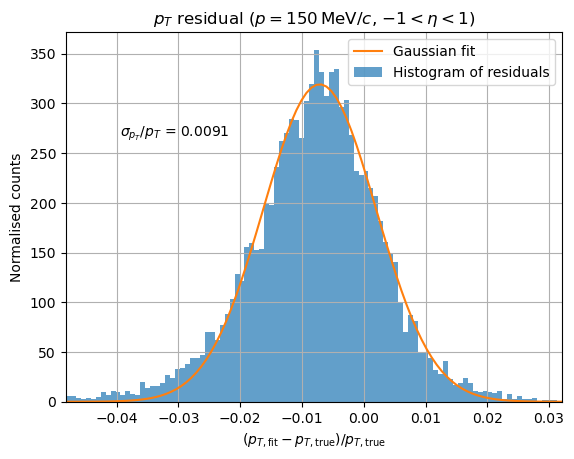
\includegraphics[width=0.7\linewidth]{gaussian_histogram_fit}
	\caption{An example of extracting the transverse momentum resolution from the Gaussian fit of the $p_T$ residuals}
	\label{fig:gaussianhistogramfit}
\end{figure}

\section{Results} \label{Results}
In this section I present the tracking resolutions obtained from the simulated single-pion samples. For each detector configuration, I generated 5,000,000 independent positive pion tracks, reconstructed the track parameters from the detector hit positions, and compared the fitted parameters with the known true values from the simulation. The quoted resolutions are the Gaussian uncertainties extracted from the residual distributions, as described in Section \ref{Measuring tracking resolution}.

\subsection{Baseline tracking resolution}
Figure \ref{fig:parametersvsp} shows the baseline tracking resolution of different tracking parameters as a function of the true momentum, for the default detector geometry, material budget, magnetic field, and hit resolution. The results are separated into different pseudorapidity bins to distinguish between the central barrel region and the forward/backward endcap regions. Here the parameter $\theta$ refers to the angle of the particle's momentum to the positive $z$-axis.

As expected from the discussion in Section \ref{Theoretical estimates of tracking resolution}, we notice different behaviours in the high and low momentum regimes for the relative momentum resolutions $\sigma_{p_T} / p_T$ and $\sigma_{p} / p$. At low momentum, the uncertainty rapidly decreases as momentum increases, being roughly inversely proportional to the momentum. This is because for low momenta, the resolution is dominated by the effect of multiple scattering, and lower momentum particles are scattered more strongly by the detector material. At high momentum, the uncertainty begins increasing linearly with the momentum. This is because for high momenta, the resolution is dominated by the intrinsic detector uncertainty, and since higher momentum particles bend less in a magnetic field, a fixed detector uncertainty results in larger fractional uncertainty in the fitted curvature.

For the resolutions of the position parameters $d_0$ and $z_0$, and the angular parameters $\phi_0$ and $\theta$, we observe that the uncertainty decreases with increasing momentum, as the track is less affected by multiple scattering.

\begin{figure}[H]
	\centering
	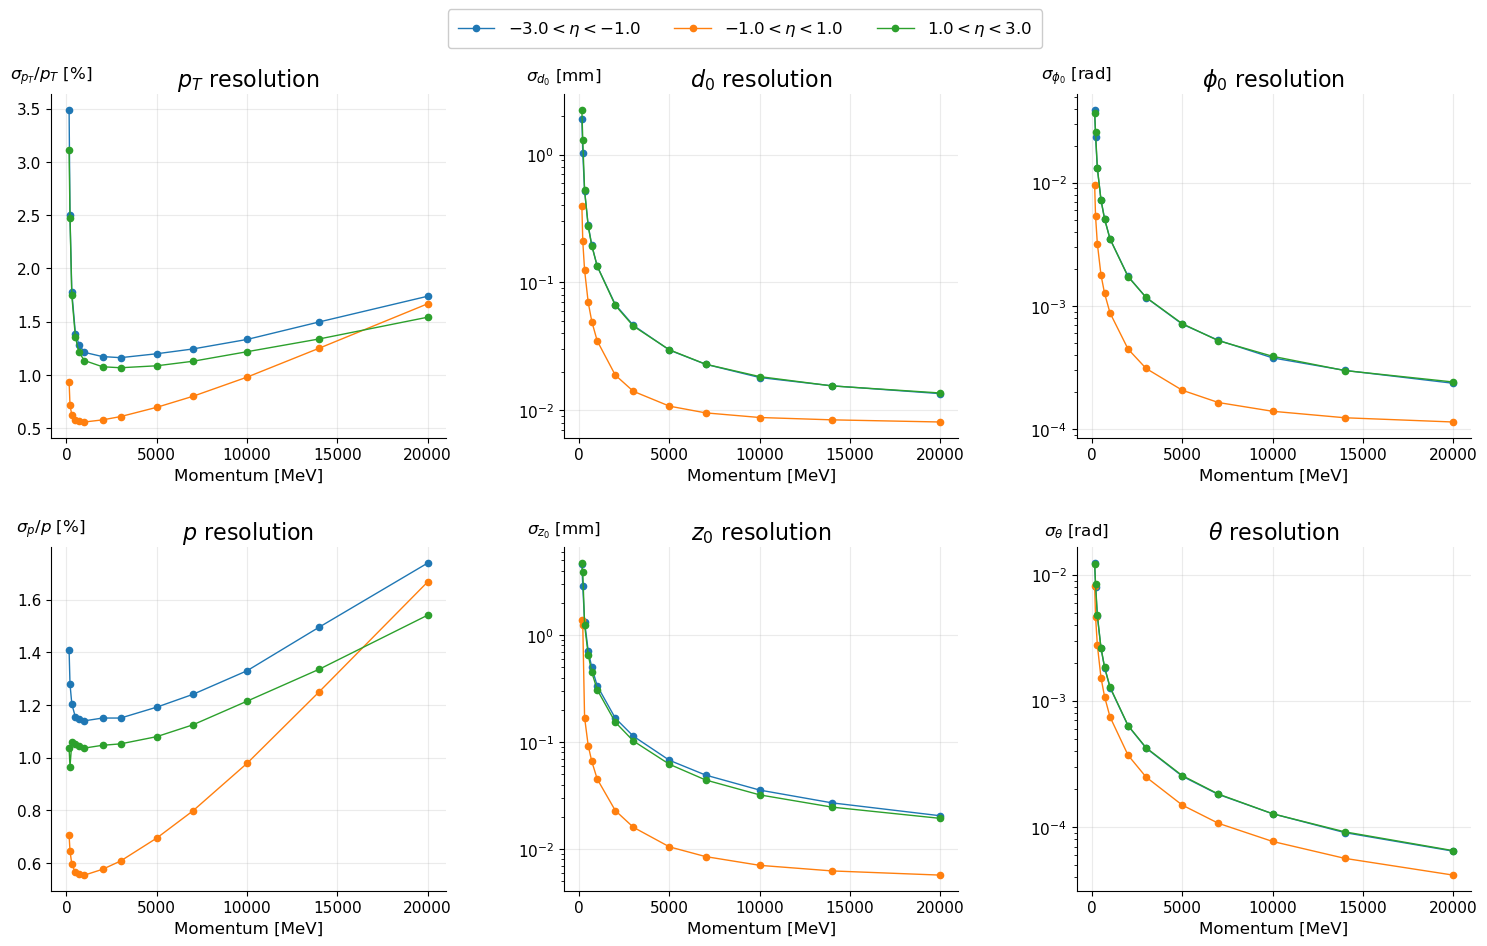
\includegraphics[width=1\linewidth]{parameters_vs_p}
	\caption{Resolution of different parameters as a function of momentum, for different pseudorapidity bins}
	\label{fig:parametersvsp}
\end{figure}

Figure \ref{fig:parametersvseta} shows the same baseline configuration, but now with the resolutions plotted as functions of pseudorapidity. The resolution for each parameter generally becomes worse at larger $|\eta|$, where particles travel at shallower angles through the detector and pass through a larger effective thickness of material. This results in more multiple scattering and reduces the precision of the fitted track parameters.

\begin{figure}[H]
	\centering
	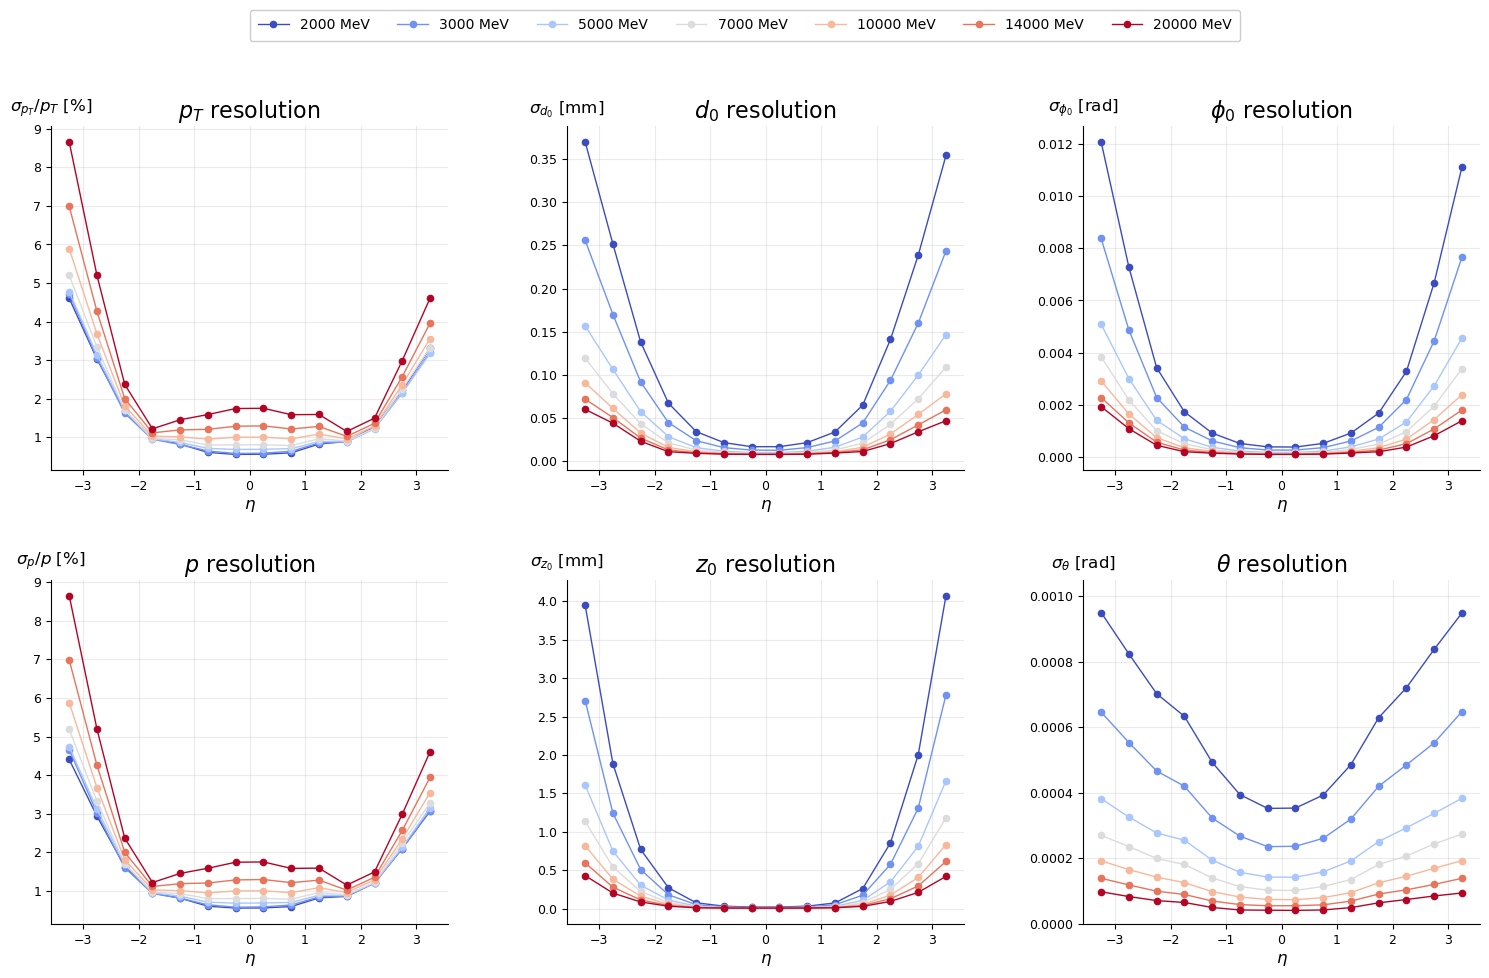
\includegraphics[width=0.95\linewidth]{parameters_vs_eta}
	\caption{Resolution of different parameters as a function of $\eta$, for different momentum values}
	\label{fig:parametersvseta}
\end{figure}

\subsection{Tracking resolution vs hit resolution}

\begin{figure}[H]
	\centering
	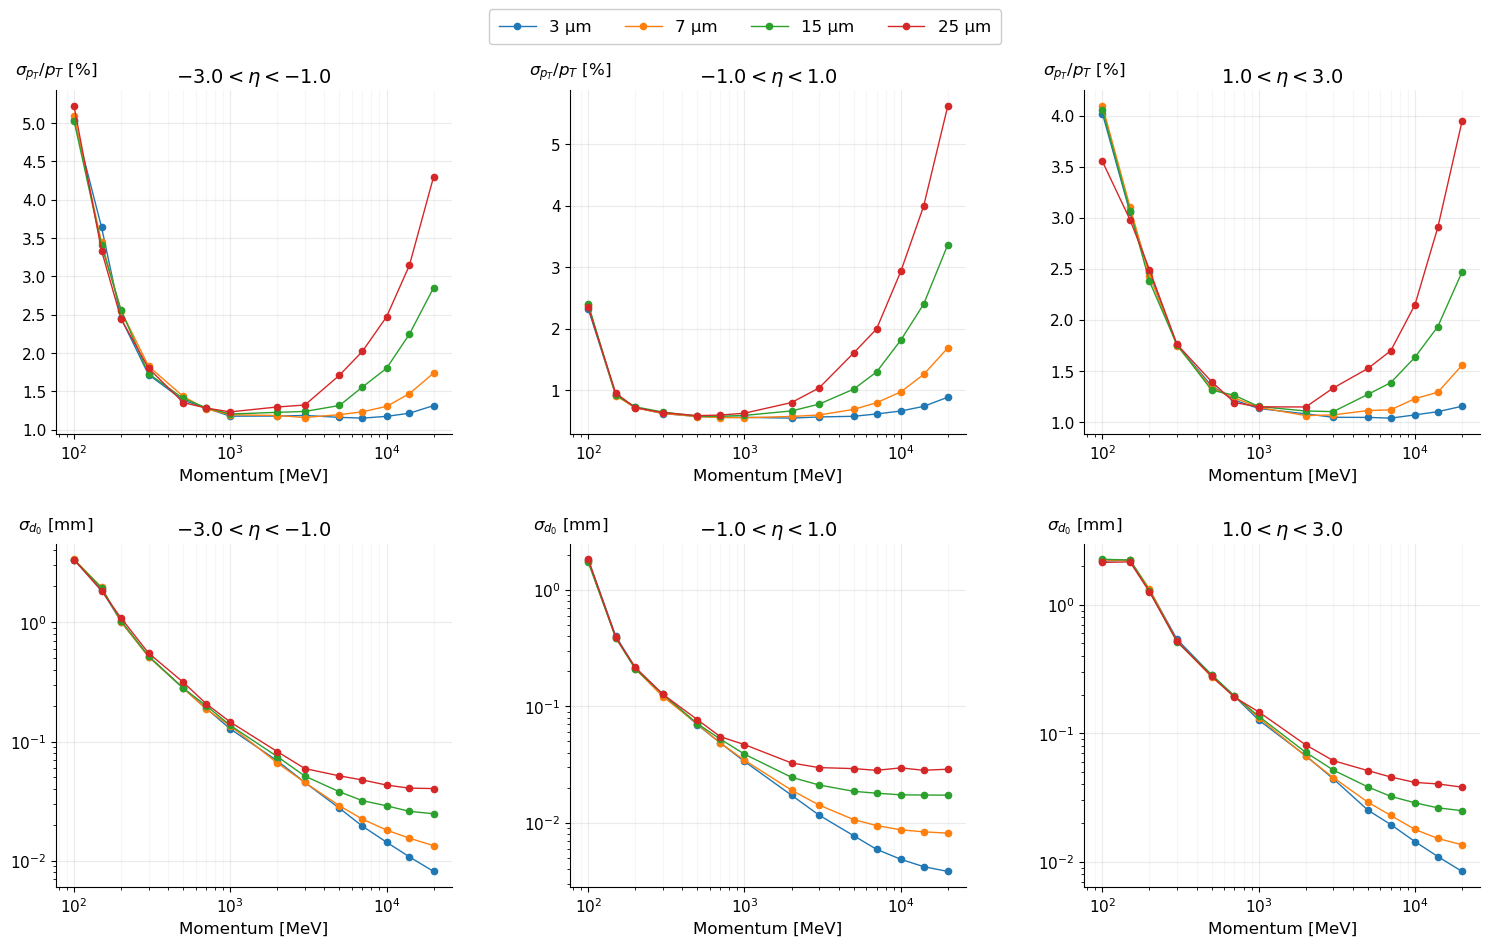
\includegraphics[width=0.95\linewidth]{resolution_vs_resolution}
	\caption{Momentum and position resolution vs momentum in different $\eta$ bins, for different values of detector resolution}
	\label{fig:resolutionvsresolution}
\end{figure}

Figure \ref{fig:resolutionvsresolution} shows the effect of changing the intrinsic hit position resolution. In the simulation, this was implemented by changing the width of the Gaussian smearing applied to detector hit positions, which is supposed to approximate the effect of changing the pixel size.

This scan is important because it tests whether improving the intrinsic sensor precision would significantly improve the final track reconstruction. At low momentum, changing the hit resolution has little effect, since the uncertainty is dominated by multiple scattering. At high momentum, the effect of intrinsic detector uncertainty begins to dominate, and so smaller hit smearing gives better momentum and vertex resolution at high momentum. Therefore we conclude that improving the intrinsic hit resolution is only useful for improving tracking performance at high momentum.

\subsection{Tracking resolution vs material thickness}

\begin{figure}[H]
	\centering
	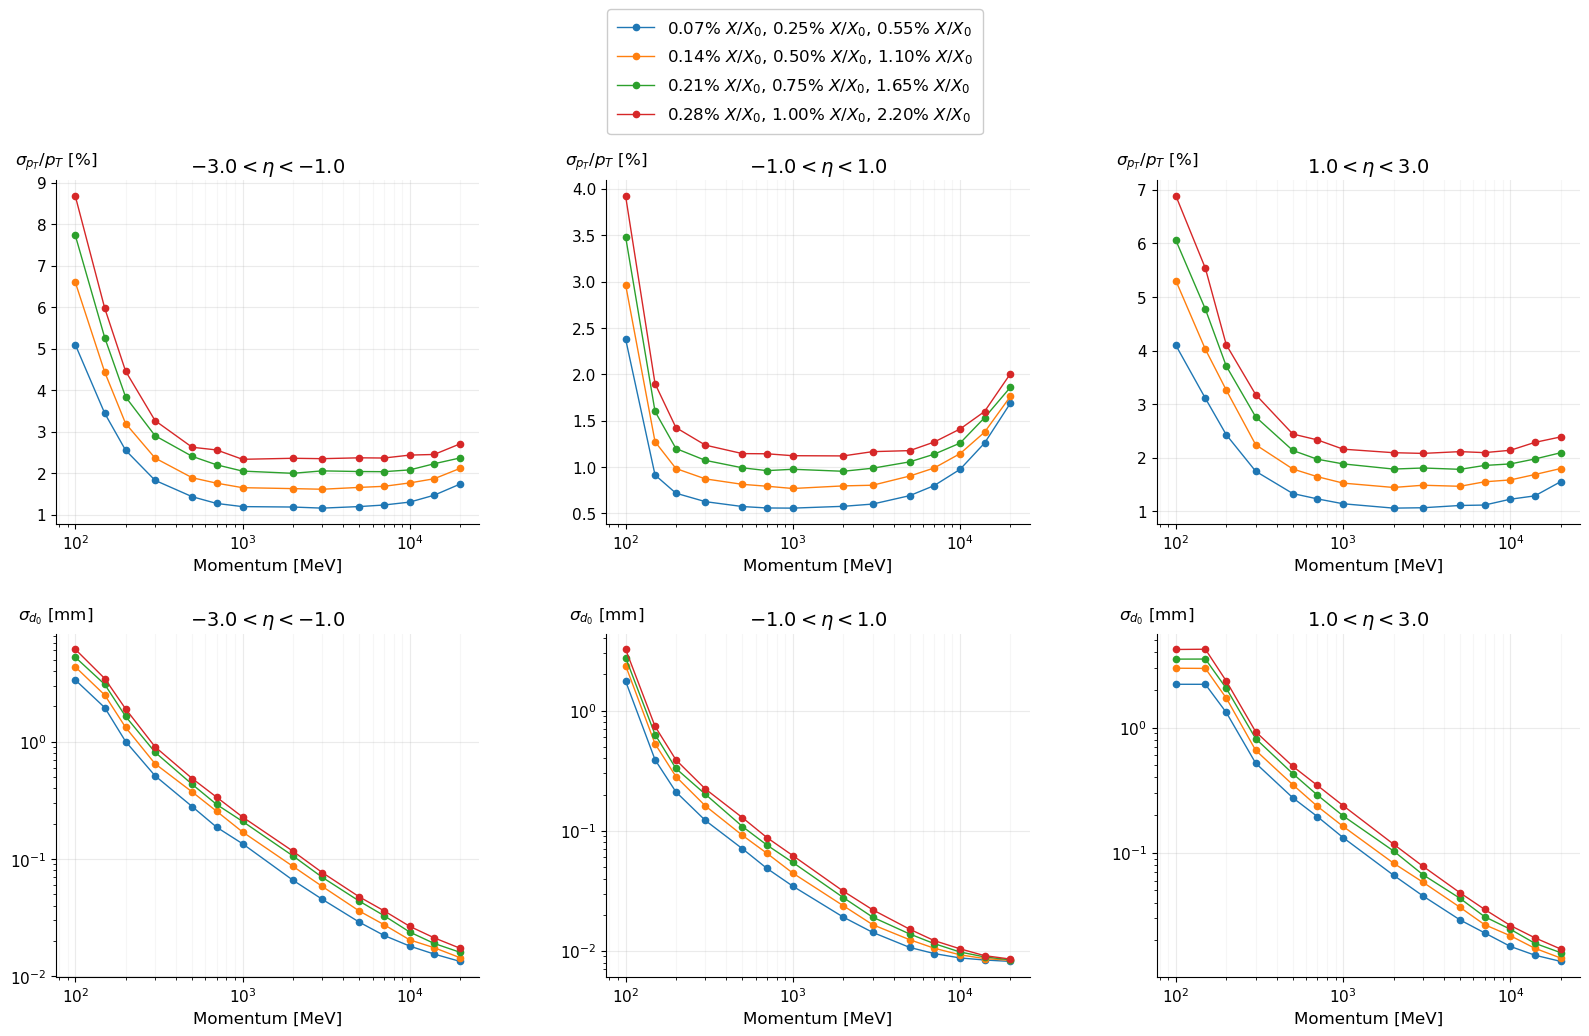
\includegraphics[width=1\linewidth]{resolution_vs_thickness}
	\caption{Momentum and position resolution vs momentum in different $\eta$ bins, for different material thicknesses}
	\label{fig:resolutionvsthickness}
\end{figure}

Figure \ref{fig:resolutionvsthickness} shows the effect of increasing the detector material budget. In this scan I kept the silicon thickness fixed at \SI{50}{\micro \metre}, and increased the thickness of surrounding support material so that the total material thickness of each layer became 1x, 2x, 3x, or 4x the baseline value\footnote[7]{
	The baseline material thickness was 0.07\% $\mathrm{X/X_0}$ per layer in the IB, 0.25\% $\mathrm{X/X_0}$ in OB layer 3 and in the endcap discs, and 0.55\% $\mathrm{X/X_0}$ in OB layer 4 \cite{turrisi2026epicsiliconvertextracker}.
} This allows the effect of adding additional electronic, support, or cooling material to be studied while keeping the silicon sensor model unchanged.

Increasing the material thickness worsens the tracking resolution across the range of momentum, with the strongest effect at low momentum due to increased scattering. The main conclusion from this scan is that minimising the material budget is one of the most important factors of detector design, since it affects tracking resolution for all momenta.

\subsection{Tracking resolution vs magnetic field}
Figure \ref{fig:resolutionvsb} shows the effect of changing the magnetic field strength. Equations \ref{eq:momentum_det_resolution} and \ref{eq:momentum_MS_resolution} indicate that increasing the magnetic field should decrease the transverse momentum uncertainty for all momenta, which is supported by the graphs. Equation \ref{eq:d0_resolution} also indicates that the magnetic field should have no effect on the position resolution, as changing the magnetic field changes the radius of curvature but not the position estimate, which is supported by the fact that no trend was seen in the resolution of the position parameters (this is not shown as there is no interesting trend).

This scan demonstrates that a strong magnetic field is important for tracking detectors, however, it is mainly useful for improving the momentum resolution and not the position resolution.

\begin{figure}[H]
	\centering
	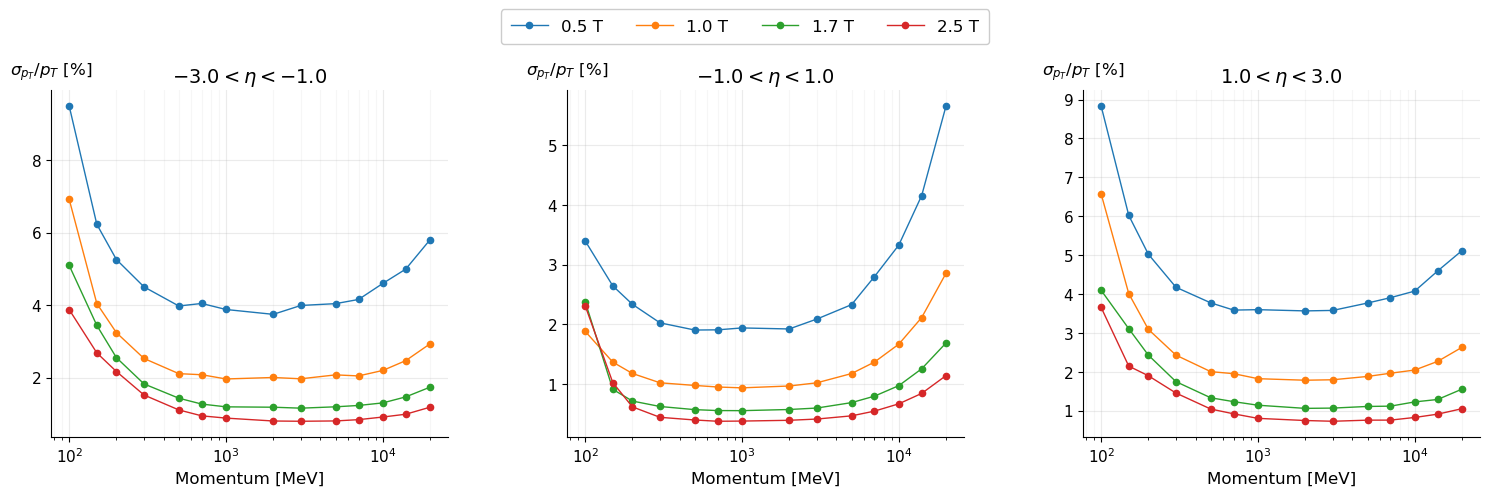
\includegraphics[width=1\linewidth]{resolution_vs_B}
	\caption{Momentum and position resolution vs momentum in different $\eta$ bins, for different values of magnetic field}
	\label{fig:resolutionvsb}
\end{figure}

\section{Conclusion}  \label{Conclusion}
The passage of pions through a simplified model of the ePIC SVT was simulated using Geant4, and helical tracks were reconstructed from hit positions in order to evaluate the momentum and position resolution of different detector designs. The baseline simulation reproduced the main expected trends in tracking performance. The position and angular parameters are measured more precisely for higher momenta, whilst the momentum resolution is split into a low momentum regime dominated by multiple scattering and a high momentum regime dominated by intrinsic hit uncertainty. Track parameters were found to be measured more precisely for low pseudorapidities, due to the particles travelling through less material and experiencing less scattering.

The momentum and position resolutions were measured after adjusting parameters of the detector design, and these results showed that one of the most important factors for detector design is minimising the material budget, as this strongly affects resolution across the entire range of momentum. A large magnetic field is also important for reducing the momentum uncertainty, but has a negligible effect on the position uncertainty. Reducing the intrinsic detector resolution is also important for precise measurements at high momentum.

There are several limitations to the computational procedure in this study. The detector geometry was heavily simplified, using idealised cylindrical barrel layers and simplified support material. The hit digitisation model was also approximate, using Gaussian smearing rather than a full simulation of charge diffusion, clustering, and pixel readout. Additionally, the reconstruction was only performed on single pion tracks with known hit associations, so the more difficult problem of track finding was not studied. Future work could use more realistic geometry, implement a more realistic digitisation model, and use track finding algorithms to study tracking efficiency and fake-track rates.

\bibliographystyle{unsrt}
\bibliography{references.bib}
	
\end{document}
